\begin{figure}[!htbp]
    \centering
    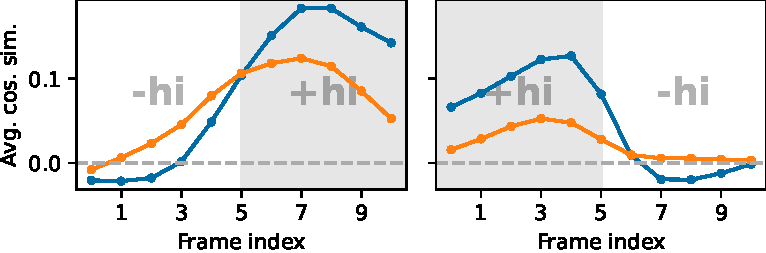
\includegraphics[width=0.9\columnwidth]{pdfs/edges-timit-wavlm-large-24-hi.pdf}
    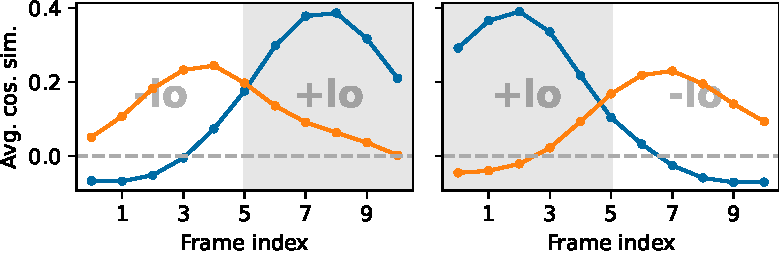
\includegraphics[width=0.9\columnwidth]{pdfs/edges-timit-wavlm-large-24-lo.pdf}
    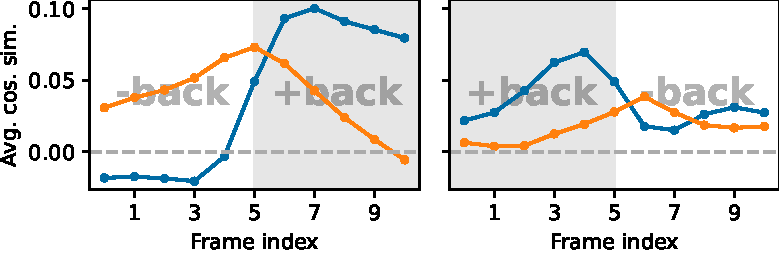
\includegraphics[width=0.9\columnwidth]{pdfs/edges-timit-wavlm-large-24-back.pdf}
    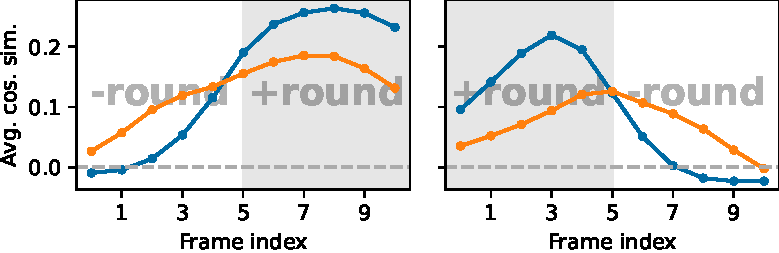
\includegraphics[width=0.9\columnwidth]{pdfs/edges-timit-wavlm-large-24-round.pdf}
    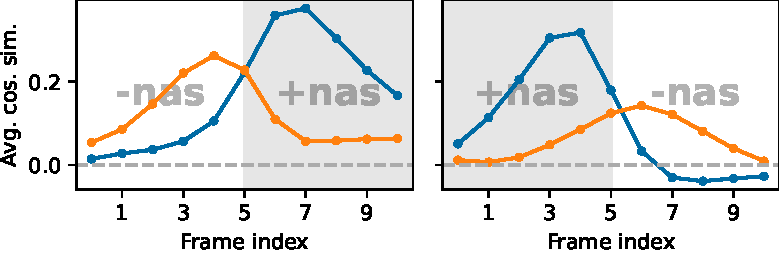
\includegraphics[width=0.9\columnwidth]{pdfs/edges-timit-wavlm-large-24-nas.pdf}
    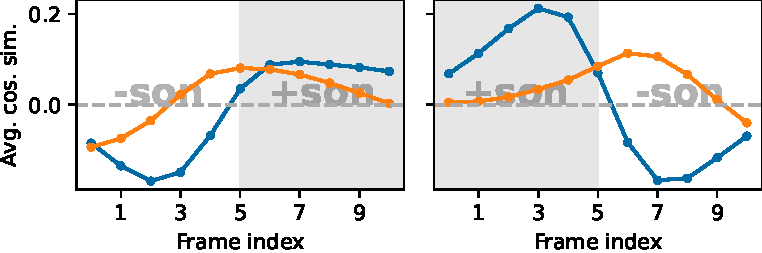
\includegraphics[width=0.9\columnwidth]{pdfs/edges-timit-wavlm-large-24-son.pdf}
    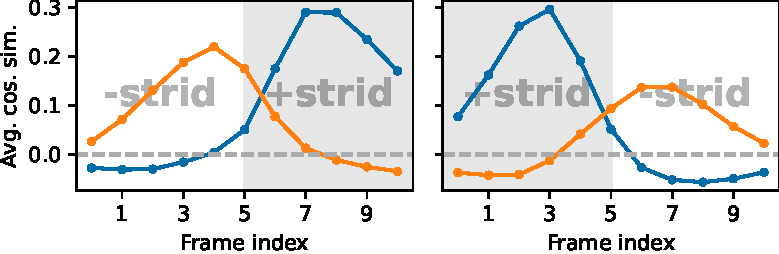
\includegraphics[width=0.9\columnwidth]{pdfs/edges-timit-wavlm-large-24-strid.pdf}
    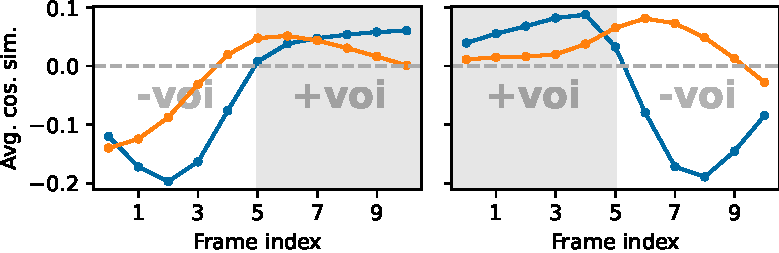
\includegraphics[width=0.9\columnwidth]{pdfs/edges-timit-wavlm-large-24-voi.pdf}
    \caption{
Phonetic segmentation experiment on TIMIT, where frame index 5 denotes the phonetic boundary of TIMIT.
Cosine similarity between frame-level S3M representations and position-dependent phonological vectors around the phonetic boundaries.
For example, for the boundary between unvoiced \texttt{[-voi]} and voiced \texttt{[+voi]}, left figure (boundary onsets) compares the evidence of current phone being voiced ($\cos(\mathbf{v}^{0}, \mathbf{r}[i])$; blue) and the following phone being voiced ($\cos(\mathbf{v}^{+1}, \mathbf{r}[i])$; orange), whereas the right figure (boundary offsets): compares the evidence of current phone being voiced ($\cos(\mathbf{v}^{0}, \mathbf{r}[i])$; blue) and the preceding phone being voiced ($\cos(\mathbf{v}^{-1}, \mathbf{r}[i])$; orange).
    }
    \label{fig:edges}
\end{figure}
